% Moved verbatim from the main text during the length revision
% (was common_body.tex lines 260-269). Content unchanged.
Feature-norm distributions differed modestly between domains. Pooled median $\|z\|$: \texttt{runA\_grl}, ISIC-test 6.31 vs.\ PAD-UFES 6.21; \texttt{runB\_orth1}, 6.38 vs.\ 6.28; \texttt{runB}, 6.28 vs.\ 5.97. At the level of pooled means, the direction was not consistent across rungs (\texttt{runA\_grl} mean: 6.72 ISIC-test vs.\ 6.83 PAD-UFES). The direction of this difference was not consistent at the level of means.

Nearest-centroid classification assigned PAD-UFES samples to the majority ISIC class (Nevus) at 61.6\% (\texttt{runA\_grl}), 61.9\% (\texttt{runB\_orth1}), and 63.9\% (\texttt{runB}), compared to 53.0\%, 53.1\%, and 53.4\% respectively for ISIC-test samples classified against their own nearest centroid. This was 8.7--10.5 percentage points higher than the ISIC-test baseline rate (ratio 1.16--1.20).

\begin{figure}[t]
\centering
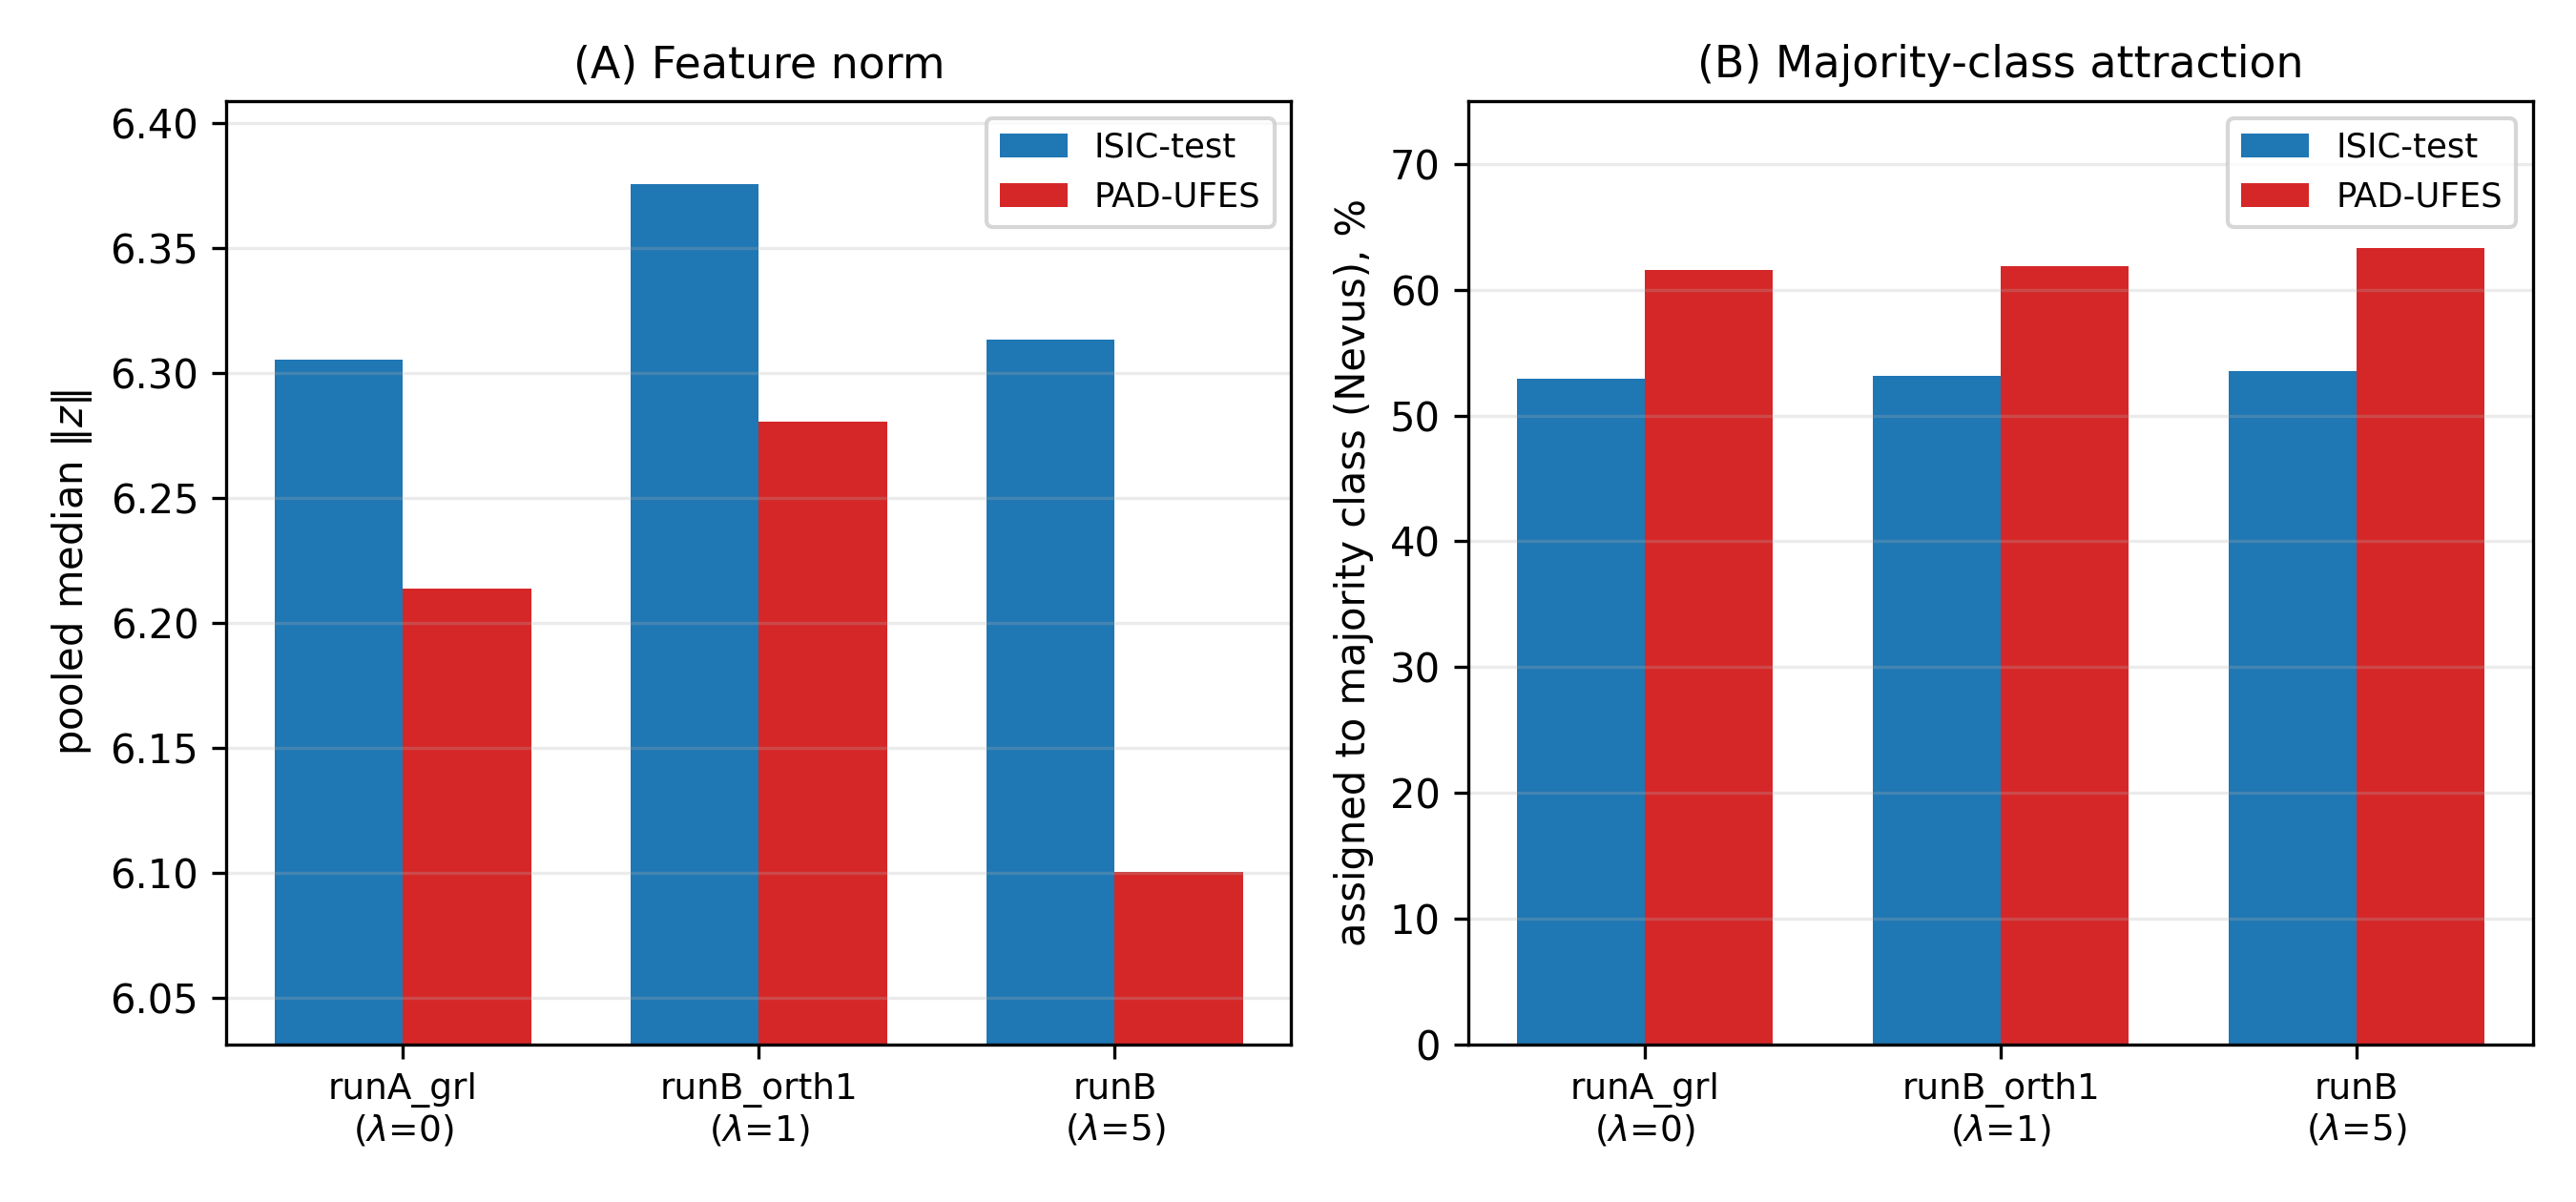
\includegraphics[width=0.9\linewidth]{figs/fig4_norm_majority.png}
\caption{Neither feature-norm difference nor majority-class attraction fully accounts for the raw ID/OOD distance gap. (A) Pooled median feature norm, ISIC-test vs.\ PAD-UFES, per rung. (B) Nearest-centroid assignment of ISIC-test and PAD-UFES samples to the majority ISIC class (Nevus), per rung. The norm difference is modest and not consistent in direction at the level of means; PAD-UFES's excess attraction to the majority class (8.7--10.5 percentage points above the ISIC-test baseline) is real but does not, on its own, account for the full distance separation in Figure~\ref{fig:geometry-vs-auroc}.}
\label{fig:norm-majority}
\end{figure}
